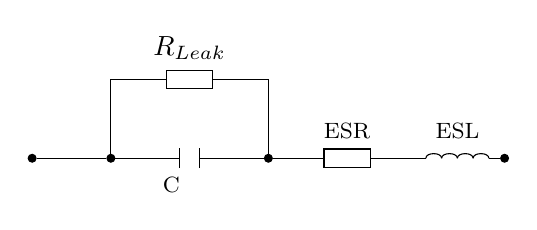
\begin{tikzpicture}

  \node (dot) at (1,1) [draw,circle,inner sep=1,fill]{};
  \node (dot2) at (2,1) [draw,circle,inner sep=1,fill]{};

  \node (c) at (3,1) [rectangle]{};
  \node (rleak) at (3,2)[draw,rectangle]{$~~~$};
  \node (dot3) at (4,1) [draw,circle,inner sep=1,fill]{};
  \node (esr) at (5,1)[draw,rectangle]{$~~~$};
  \coordinate (eslstart) at (6,1);
  \coordinate (eslend) at (6.8,1);
  \node (esl) at (6,1)[rectangle]{};
  \node (dot4) at (7,1) [draw,circle,inner sep=1,fill]{};

  \draw (dot) -- (dot2) -- (c) -- (dot3) -- (esr) -- (eslstart) (eslend) -- (dot4);
  \draw (dot2) |- (rleak) -| (dot3);

  \draw (c.south west) -- (c.north west);
  \draw (c.south east) -- (c.north east);

 \begin{scope}[out=90,in=90]
   \foreach \x in {0,0.2,0.4,0.6}
      \draw (eslstart)++(\x,0) to ++(0.2,0);
 \end{scope}

 \draw (rleak.north) node[above]{$R_{Leak}$};
 \draw (esr.north) node[above]{\footnotesize ESR};
 \draw (esl.north) node[above right]{\footnotesize ESL};
 \draw (c.south) node[below left]{\footnotesize C};


\end{tikzpicture}
